\begin{center}{ \bf К МОДЕЛИ СВЕТОВОГО ПРОЦЕССОРА}\\
{\it А.А.Игнатьев, Е.И.Яшагин} \\
(Зеленодольск; {\it eugene.yashagin@gmail.com})
\end{center}
\addcontentsline{toc}{section}{Игнатьев А.А.,Яшагин Е.И.\dotfill}

Рассмотрим пучок прямых первого рода и примем физическое условие: угол падения равен углу отражения.
Обозначим общую точку прямых (их точку пересечения) за $M_0\left(x_0;\ y_0\right)$.
Наша задача -- нахождение кривой,
состоящей из точек пучка на которых выполняется условие отражения из фиксированного источника в фиксированный приёмник.
Пусть $S$ и $P$~--- точки источника и приёмника соответственно. Поместим $S$ в $O$--  начало координат, $P\in OX$.

На каждой прямой пучка существует точка (обозначим её за $M\left(x;y\right)$), такая что угол между радиусом-вектором $\overrightarrow{r}=\left\{x;y\right\}$ к ней и вектором нормали $\overrightarrow{N}$ к прямой в точке $M\left(x;y\right)$ будет равен углу между вектором $\overrightarrow{PM}$, соединяющим точку $P\left(p;0\right)$, принадлежащей координатной прямой $OX$, с точкой $M$ и вектором указанной нормали$\overrightarrow{N}$.

Зададим в искомой точке отражения на прямой пучка направляющий вектор $\overrightarrow{a}=\left\{x-x_0;y-y_0\right\}$. $\left(\overrightarrow{a},\overrightarrow{N}\right)=0$, так как они перпендикулярны. Если $\overrightarrow{r}=\left\{x;y\right\}$ и $\overrightarrow{PM}=\left\{x-p;y\right\}$, то  $\overrightarrow{N}=\frac{1}{\sqrt{x^2+y^2}}\left\{x;y\right\}+\frac{1}{\sqrt{{\left(x-p\right)}^2+y^2}}\left\{x-p;y\right\}$. Отсюда, $\left(\overrightarrow{a};\overrightarrow{N}\right)=\left(\overrightarrow{a},\frac{\overrightarrow{r}}{\left|\overrightarrow{r}\right|}+\frac{\overrightarrow{PM}}{\left|\overrightarrow{PM}\right|}\right)=0$ или в координатах:
\begin{multline*}
	\sqrt{{\left(x-p\right)}^2+y^2}\left(x(x-x_0)+y(y-y_0\right))=
	\\=
	\sqrt{x^2+y^2}\left(\left(p-x\right)\left(x-x_0\right)-y\left(y-y_0\right)\right)
\end{multline*}
Это есть уравнение кривой, состоящей из точек, удовлетворяющих условию отражения.

Под отражением здесь мы понимаем не только физическое отражение, когда перпендикуляр к прямой образует равные углы с $\overrightarrow{r}$ и $\overrightarrow{PM}$ по одну сторону от прямой, а также и случай, когда это вертикальные углы. Тогда справедливо следующее утверждение.

\textbf{Теорема 1.}
Для любых двух точек $S$ и $P$ и любого собственного пучка прямых с общей точкой $M_0$ множество точек отражения на прямых пучка есть замкнутая кривая, включающая в себя точку $M_0$ и отрезок $SP$.

Замечание. На отрезке $SP$ не выполняется условие физического отражения и обычно такие точки исключаются из рассмотрения [1], но на практике это просто прямой ход луча из источника\textit{S} вприёмник \textit{P}.

Наши исследования выявляют четыре варианта вида кривой, в зависимости от числа пересечений с координатными осями при указанном выше выборе координат источника\textit{S} и приёмника\textit{P}.

\begin{figure}
	\centering
	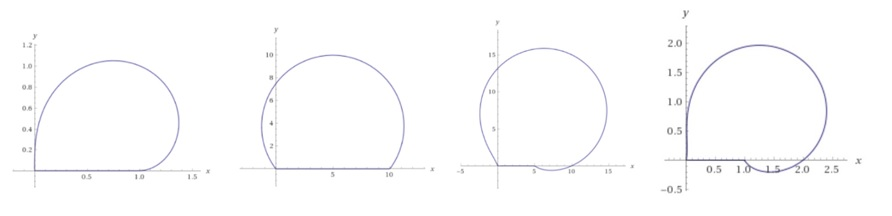
\includegraphics[width=0.9\linewidth]{Ignatev.jpg}
\end{figure}

Решая нашу задачу в пространстве, мы получаем уравнение поверхности:
%
\begin{multline*}
	\sqrt{{\left(x-p\right)}^2+y^2+z^2}\left(x\left(x-x_0\right)+y\left(y-y_0\right)+z\left(z-z_0\right)\right)=
	\\=
	\sqrt{x^2+y^2+z^2}\left(\left(p-x\right)\left(x-x_0\right)-y\left(y-y_0\right)-z\left(z-z_0\right)\right)
\end{multline*}

В плоскости, задаваемой точками $S,\ P$ и $M_0$, мы всегда получаем замкнутую кривую, включающую отрезке $SP$. В то же время в пространстве поверхность, где выполняется условие физического отражения, можно охарактеризовать следующим образом.

\textbf{Теорема 2.}  Существует такая плоскость, содержащая отрезок $SP$ и не содержащая точку $M_0$, которая разбивает всё пространство на две части: в том полупространстве, где лежит точка $M_0$, находится ограниченная часть поверхности, а в оставшемся полупространстве поверхность отражения неограниченна, причём поверхность ограниченной части имеет минимальную площадь поверхности.

Это утверждение может иметь практическое применение при использовании найденной поверхности
для нового варианта модели реализации светового процессора.
Рассмотрение разных
\linebreak
расположений точки в пространстве есть ключ к исследованию поведения поверхности отражения,
при этом как в целом, так и ограниченной её части сечением указанной выше плоскости
и условия минимальности площади поверхности этой ограниченной части [2].

В трёхмерном случае для практических приложений важным является нахождение множества точек, в которых невозможно отражение для любой поляризации падающего луча [3], [4]. Это требование применительно к нашей задаче можно выразить аналитически следующей формулой:

\[\left[\overrightarrow{M_0M},\ \left[\overrightarrow{SM},\overrightarrow{PM}\right]\right]=\overrightarrow{O}\]

Расписывание этого выражения в координатах даёт систему из трёх уравнений, каждое из которых описывает некоторую поверхность второго порядка, вид которой зависит от параметра \textit{p}, и координат точки \textit{M0}--  \textit{x0, y0, z0}. Совместное решение даёт искомое множество точек.
Заметим также, что в найденных нами точках полного неотражения для любой поляризации, в частности, выполняется и условие известного закона полного преломления для плоско поляризованного луча.

\smallskip \centerline{\bf Литература}\nopagebreak

1. {\it Брус Дж., Джиблин П.} Кривые и особенности -- Москва: Изд-во «Мир», 1988, 262с.

2. {\it Джусти Э.} Минимальные поверхности и функции ограниченной вариации -- Москва: Изд-во «Мир», 1989, 239с.

3. {\it Сивухин Д. В.} Общий курс физики. -- Москва: Изд-во «Наука», 1980 -- Т. IV. Оптика, 752с.

4. {\it Борн М., Вольф Э.} Основы оптики. --  М.:Изд-во «Наука», 1973.,713с.
